\chapter{Cross-Validation}
\label{chap:crossval}
Advanced machine learning algorithms typically come with a set of hyper-parameters, \eg{}, the $C$ and $\gamma$ parameter of \glspl{svm} or the number of trees in a random forest that are fixed before the learning process begins and are not objective of the training process itself.
The choice of these values can impact the performance of the trained model and help convergence, yet optimal values are unknown a priori. 
In a canonical approach one splits a second test set and uses it to optimize the hyper-parameters since optimizing on the training (test) set could seed overfitting\footnote{Especially when scanning the hyper-parameter space exhaustively, this problem is similar to the so-called \textit{look elsewhere effect}~\cite{lookelsewhere}.} (selection bias) which clearly comes by the costs of a reduced training set.
Cross-validation (\eg{}, Refs.~\cite{crossval1,crossval2}) is an alternative technique that allows to optimize hyper-parameters on the training set without suffering from overfitting.
In the present analysis we use a 5-fold cross-validation scheme where the training set is partitioned into five, equally sized folds (\cf{}~Fig.~\ref{fig:apdx_crossval}).
Hyper-parameters are optimized on each of these folds by training the classifier on four and evaluated on the last fold (4+1).
The loss of accuracy in terms of a large uncertainty due to the small sample size of each of the folds used for the evaluation is compensated by combining the results of the five independent folds.
\begin{figure}[htbp]
    \centering
    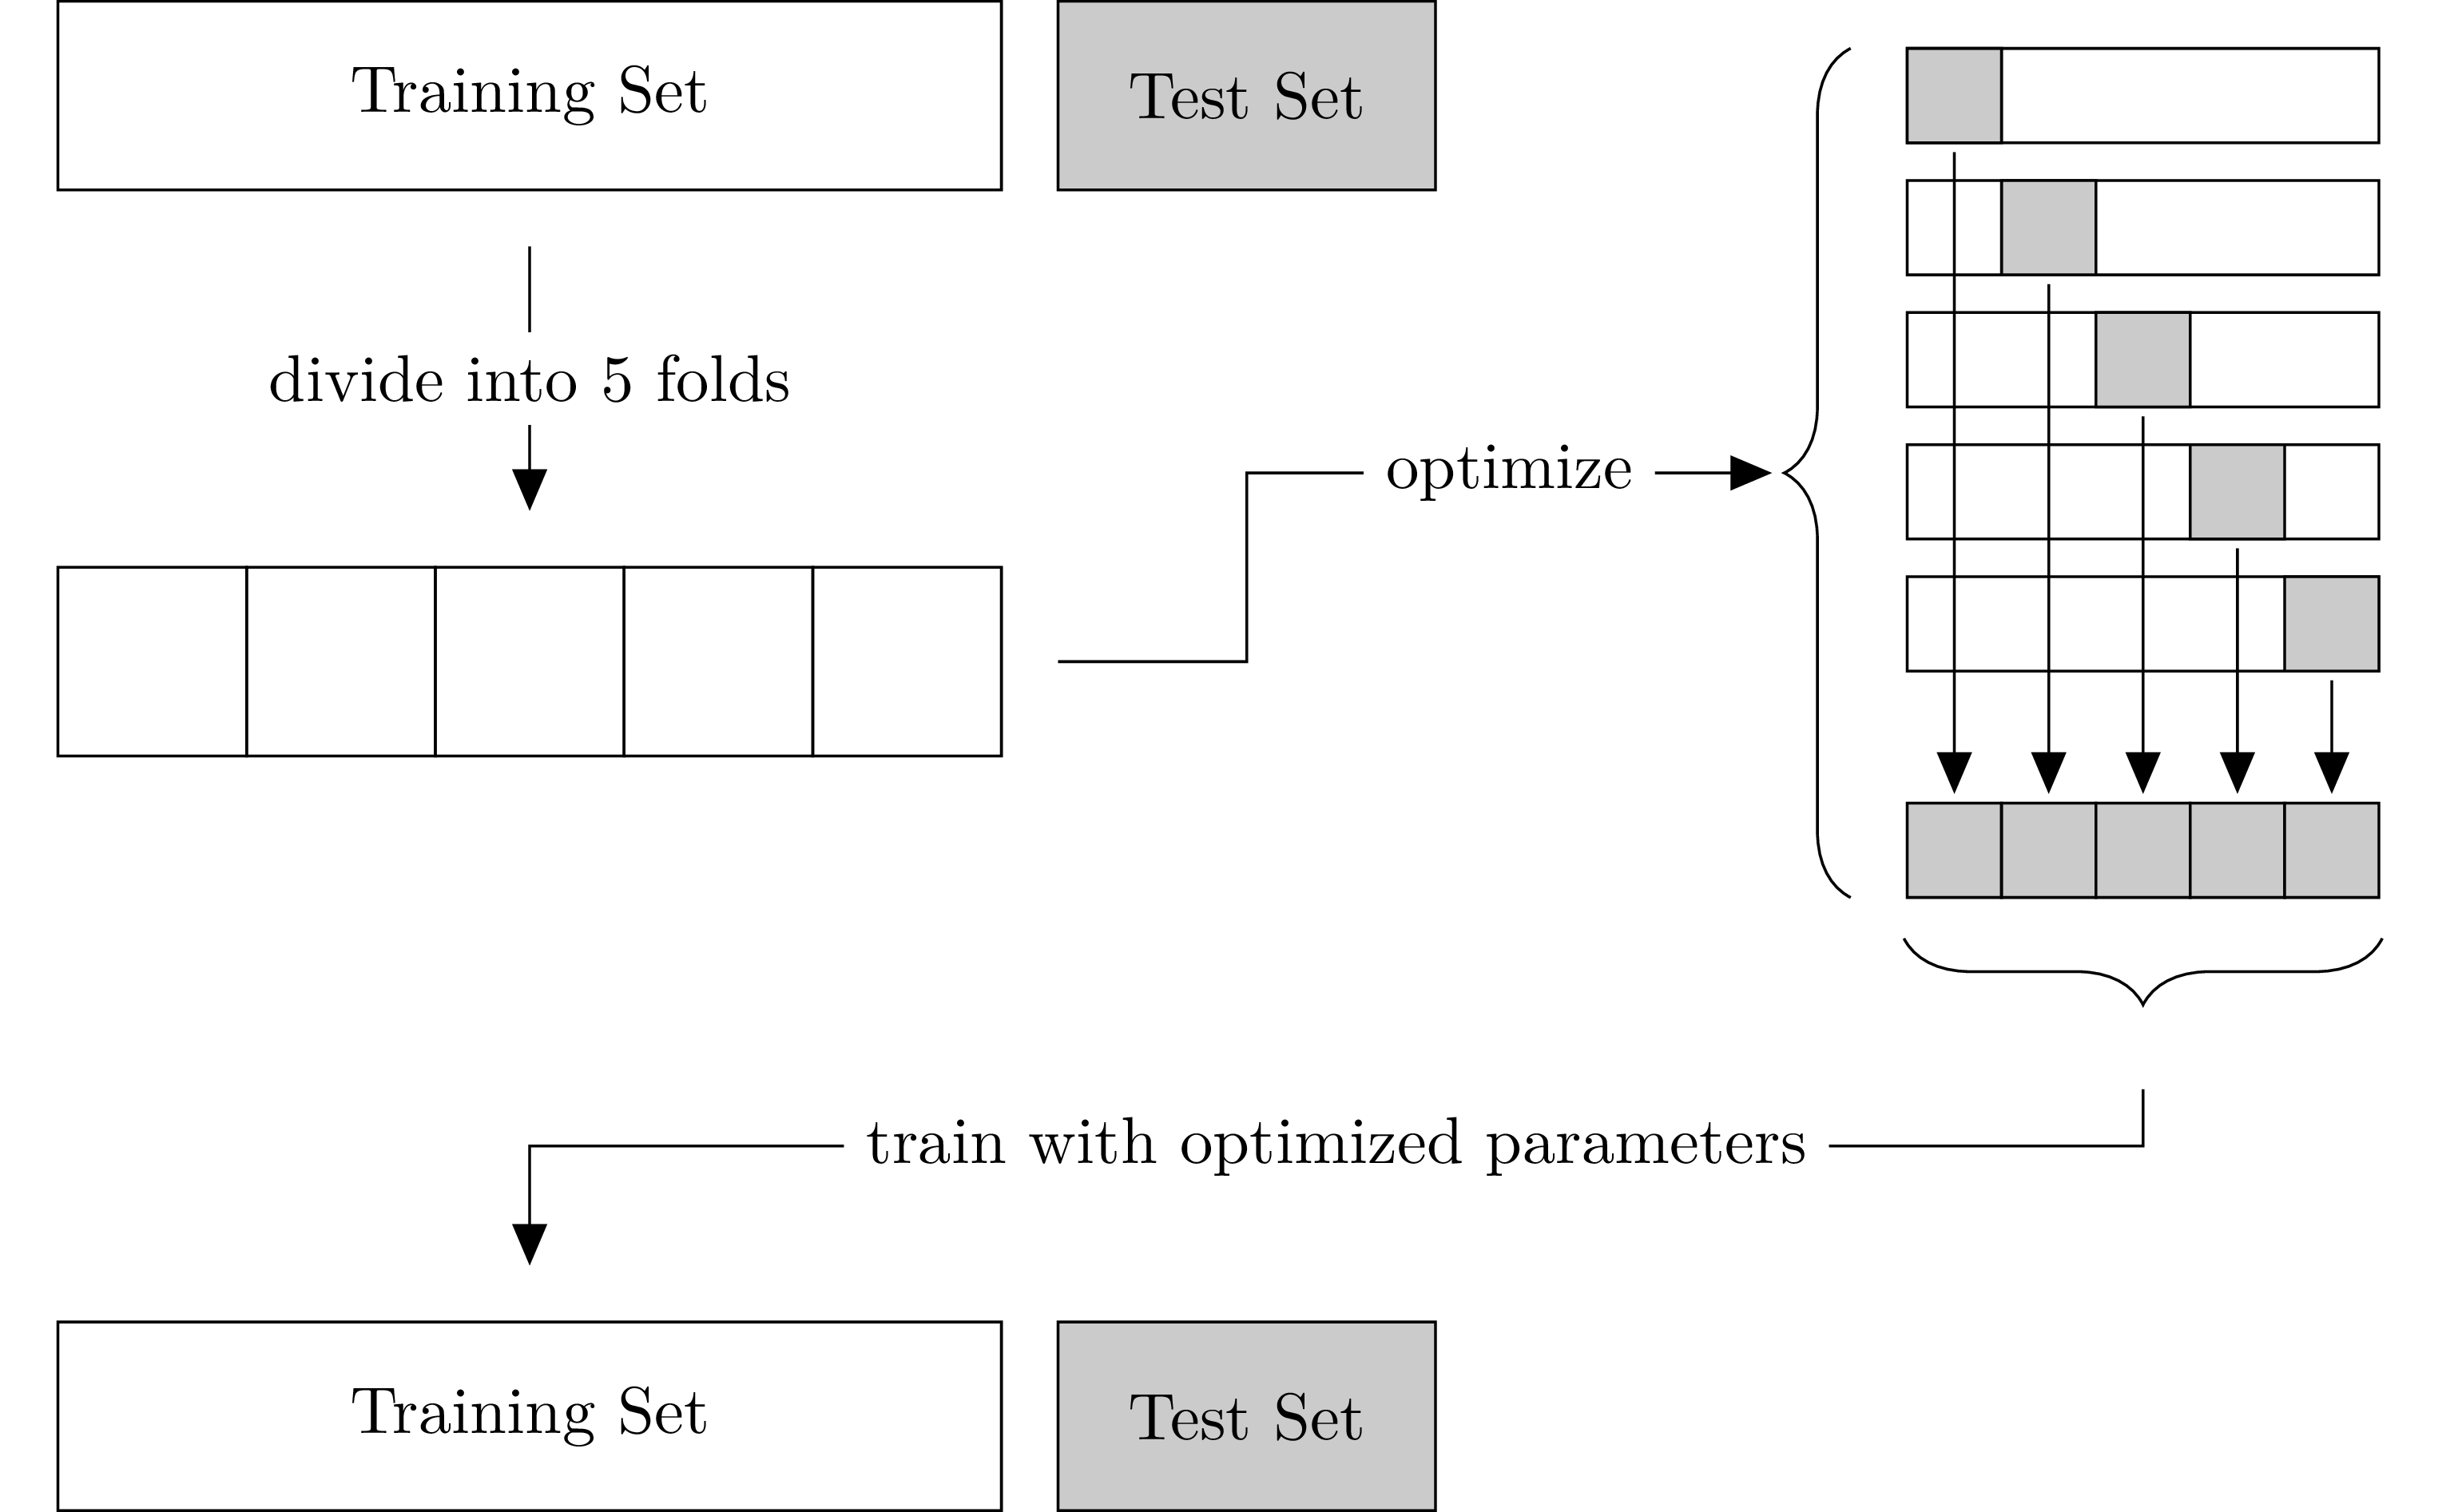
\includegraphics[scale=1.]{apdx_crossval/crossval.png}
    \caption{Outline of a 5-fold cross-validation where hyper-parameters are optimized on folds of the training set instead of the test set.}
    \label{fig:apdx_crossval}
\end{figure}

